\documentclass[10pt,twocolumn,letterpaper]{article}
%% Language and font encodings
\usepackage[english]{babel}
\usepackage[utf8x]{inputenc}
\usepackage[T1]{fontenc}
% xcolor is the package between braces and between brackets is the option that we want to use
\usepackage{fancyhdr}
\usepackage{biblatex}
\usepackage{array}
\usepackage[color]{showkeys}
\usepackage{etoolbox}
\usepackage{graphicx,tabularx}
\usepackage{amsfonts} 
%% Sets page size and margins
\usepackage[a4paper,top=3cm,bottom=2cm,left=3cm,right=3cm,marginparwidth=1.75cm]{geometry}
%% Useful packages
\usepackage{amsmath}
\usepackage[colorlinks=true, allcolors=blue]{hyperref}
\fancypagestyle{plain}{%
  \fancyhead{}
  \fancyfoot{}
  \fancyfoot[R]{\thepage}
  \fancyfoot[L]{[INFOMR] Multimedia Retrieval - Utrecht University}
}
\pagestyle{plain}
\title{%
  3D Mesh Retrieval System \\
  \large Multimedia Retrieval \\
    Utrecht University}
    
\author{
  Da Costa Barros, Fabien [0720823]\\
  \url{f.n.dacostabarros@uu.students.nl}
  \and
  Bagheri, Soheil [6208908]\\
  \url{s.bagheri@students.uu.nl}
}
\date{\today}
\addbibresource{refs.bib}                                                                     
\begin{document}
\maketitle
\selectlanguage{english}
\section*{Introduction}
With the advance in modeling software and 3D scanners, the speed of 3D content creation increased rapidly. Nowadays, much 3D content has been produced, and people are still creating many more objects constantly. These kinds of contents are usually stored in so-called shape databases. But, there is a challenge to browse and find the 3D objects of interest within these numerous amounts of data.\\ \\
Several techniques have already been presented for finding desired data in these shape databases. For example, searching by keyword, browsing the database along a few predefined categories, or content-based shape retrieval (CBSR). Although the first two options do not need a sample model for searching in a database, they need more effort to label or categorize these contents. On the other hand, there is content-based shape retrieval which can retrieve all the similar samples to the existing query shape.\\ \\
In this project, we want to categorize the 3D objects of a database based on their shape similarity. This process will be done by normalizing all the objects and extracting some general features from them. Then, we can divide similar objects based on their similarity in their features. Also, there would be a content-based shape retrieval that can find similar 3D objects based on the feature extracted from the given query shape and compared to other objects in the database.

\section{Selection and setup the work environment}
In this section, four different related packages have been tested and compared. The Comparison of these packages has been done based on several features that might be useful in the future sections of this project. For example, being able to re-mesh objects, scaling them, rotating them, and moving them are the feature that can be useful in the process of normalizing the 3d objects in the database. Also, having some information about the 3d objects, like the number of vertices and faces, is necessary for understanding if these 3d objects are normalized or not. On the other hand, this package must support different formats that are usually used to store 3d objects.
In this case, we narrowed down the packages that work with Python language and well-known between the community. So, we tested and analyzed "Pymesh", "PyMeshLab", "TriMesh", and "Open3D". Results can be found in the table 1.\\ \\
We wanted to be able to open "PLY", "OFF", "OBJ", and "STL" formats. "PLY" and "OFF" formats were discussed in the lecture, while "OBJ" and "STL" are really common. All of them were able to open "PLY", "OFF", "OBJ", and "STL" formats, so that was not really discriminating. \\ \\
	We tried to compare the different re-meshing, repairing and extraction features with our current knowledge and thought that PyMeshLab and Open3D seems to be quite good. The complexity was also one of our requirements as from previous experience less complex library offers less options. \\ \\
	After achieving step 1 with four of those libraries, we try to find a balance between number of dependencies, options proposed for visualizing and analysis. Then we decide to choose "PyMeshLab"\cite{pymeshlab}
Our project has three main dependencies. "PyMeshLab", "Polyscope", and "Numpy", and it runs with Python 3.9. \\ 
\begin{table*}[ht]
    	\hspace*{-0.1\linewidth}\begin{tabular}{|p{0.25\linewidth}|p{0.2\linewidth}|>{\centering}p{0.15\linewidth}|>{\centering}p{0.15\linewidth}|>{\centering}p{0.15\linewidth}|>{\centering\arraybackslash}p{0.15\linewidth}|}
    		\hline
     		Features category & Desired Fetures & PyMesh & PyMeshLab & TriMesh & Open3D \\ \hline
    	    3D format supported & PLY & X & X & X & X \\
    	    ~ & OFF & X & X & X & X \\
    	    ~ & OBJ & X & X & X & X \\
    	    ~ & STL & X & X & X & X \\ \hline
    	    Repairing & Isolated Vertices & X & X & X & To implement \\ 
     		~ & Duplicated Vertices & X & X & X & To implement \\ 
    	    ~ & Duplicated Faces & X & X & X & To implement \\ \hline
    	    Remeshing & Uniform sampling & X & X & X & X \\ \hline
    	    Analysis features & ~ & Simple & Rich & Sufficient & Rich \\ \hline
    	    Visualisation features & Scale & 0 & X & X & X \\ 
   		    ~ & Pan & 0 & X & X & X \\ 
     		~ & Rotate & 0 & X & X & X \\
        	~ & Screenshot & 0 & X & 0 & X \\ 
        	~ & Multiple mesh & 0 & X & 0 & X \\ \hline
        	Language & Source code & 70\% C++ \newline 20\% Python \newline 10\% C  & 80\% C++ \newline 20\%Python & 100\% Python & 80\% C++ \newline 10\% Python \newline 10\% Cuda \\ \hline
        	Number of dependencies & ~ & 7 & 2 & 3 & 0 \\ \hline
        	Interface of preview windows & ~ & None & Advanced & Minimalistic &~ \\ \hline
        	Visualisation interface & Shading methods & None & Flat & Flat & Flat \\ \hline
        	Installation tools & Pip or Anaconda & Docker & Pip & Pip & Pip \\ \hline
    	\end{tabular}
    	 \caption{In-built features for different Python libraries}
  		\label{tab:libraries}
	\end{table*} \\ \\


\section{Rendering}
We have two scripts for this step called "main.py" and "render.py" Where "main.py" verifies the console arguments and calls the render function from "render.py". The first argument passed through is the path of the file. \\ \\
In "render.py", there is a function called "render". This function loads the mesh and displays the vertices and the mesh of the 3D object. PyMeshLab has a built-in function ".show\_polyscope" that shows a mesh. While we found it more interesting to override it with polyscope functions to have more control if we need to upgrade anything. The result of the mesh visualization script can be found in Figure \ref{fig:ant-mesh}. The 3D mesh visualization windows offered many functionalities.

\begin{figure}[h!]
\begin{center}
  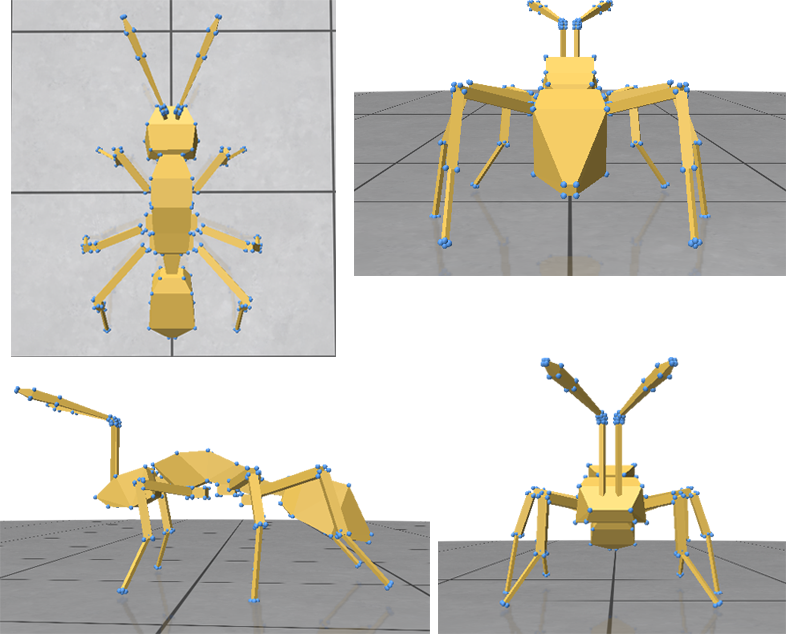
\includegraphics[width=0.5\textwidth]{picture/ant}
  \caption{Visualisation of an ant mesh}
  \label{fig:ant-mesh}
  \end{center}
\end{figure}

\section{Shape analysis}
To avoid too many disparities between several meshes in the database, we wanted to normalize some features of the database we implemented a function to retrieve generic information from a mesh. Towards the idea of normalizing the number of vertices, the position, the scale, the alignment, and the orientation. We have implemented a filter to retrieve the number of vertices, barycenter, the size of the bounding box, the vector given by principal component analysis, and the second-order moment of mass.
	
	We have to determine an order for all the different steps as a transformation can have an impact on the following one. Mainly any transformation T has to be performed before T' if T have a side effect on the property that T' normalize. First of all, we begin with the numbers of vertices to obtain a uniform description of the shape of the poorly sampled mesh. This makes some computation easier as we can assume that each vertex describes the same amount of mass. In the first place, we normalize the position as it does not impact any other properties. We remark that any rotation impacts the size of the bounding box and the flipping so we compute alignment with the axis given by PCA in second place and the flipping in third place as both are a matter of rotation. In the fourth place, we scale the mesh to the unit cube as it will not influence any of the previous properties (namely the position, scaling, or alignment with the most spread axis given by PCA). The flipping operation or scaling operation don't influence each other so we could have computed the last two transformations in a different order.
	
We will go into further detail, analyzing the descriptors for each feature now.


\subsection{Vertex numbers}
\label{subsec:vertex numbers}

\subsection{Position}

One way of normalizing the position is to translate the barycenter at the origin of the 3D spaces. PyMeshLab have an in-built function made for this. Here is one way to implement such functionalities, first the barycenter of the mesh needs to be computed. To compute this we have to compute the average position of the center of all faces weighted by the area of the face. Each vertex doesn’t describe the same amount of mass, in particular, if the vertices are non-uniformly distributed over the mesh.  Although if the repartition of the vertex is uniform (as we ensured in section \ref{subsec:vertex numbers}), we assume that each vertex represents the same amount of mass. This assumption made we can just compute the average x,y, and z of all the vertex of the mesh. Here is the formula to compute the barycenter the i-th coordinate of the barycenter ($i \in \{x,y,z\}$) :

$$ b_i = \frac{\sum_{v \in V} v_i}{|V|}  $$ (with i the i-th coordinate of v ($i \in \{x,y,z\}$)and V the set of vertex of the mesh.)
	
	Once the barycenter is computed we just translate each vertex by the $\overrightarrow{BO}$ vector (with B the barycenter and O the origin of the 3D reference space). We can compare the distance of the barycenter to the origin for each mesh before and after normalization.
	
\begin{figure}[h!]
\begin{center}
  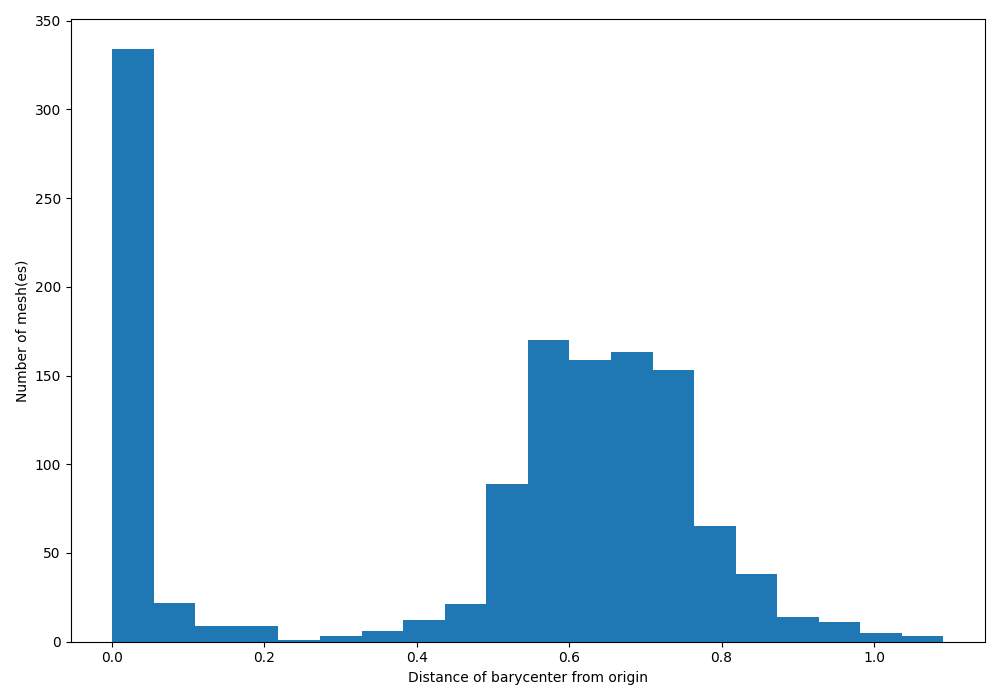
\includegraphics[width=0.5\textwidth]{picture/Initial barycenter}
  \caption{Position of the barycenter to the origin for the initial 3D mesh database}
  \label{fig:barycenter-before}
  \end{center}
\end{figure}

\begin{figure}[h!]
\begin{center}
  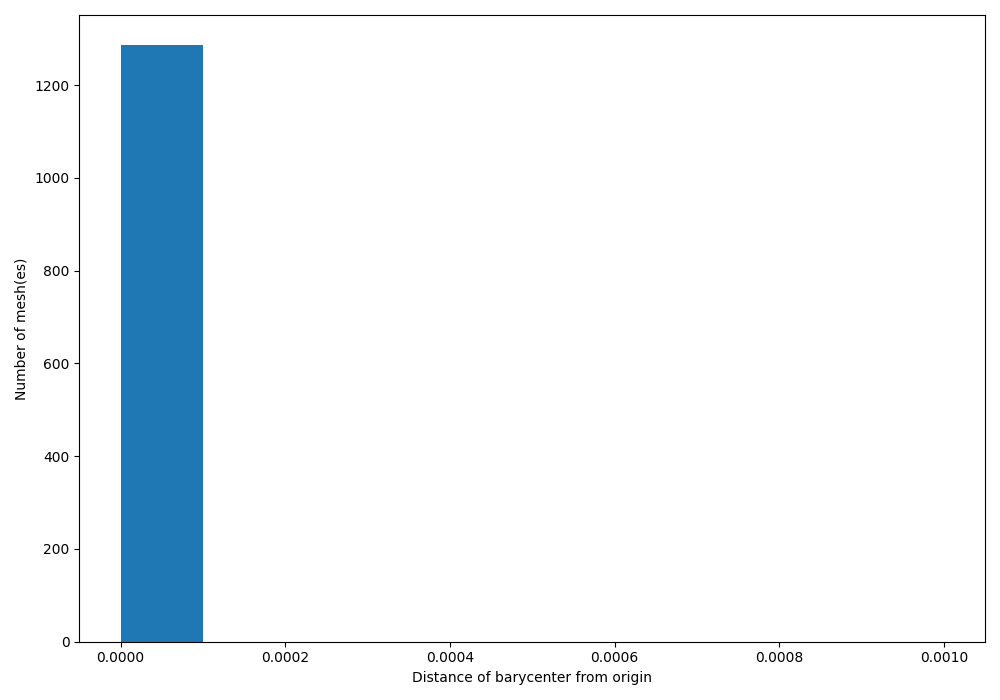
\includegraphics[width=0.5\textwidth]{picture/Normalised barycenter}
  \caption{Position of the barycenter to the origin after normalisation}
  \label{fig:barycenter-after}
  \end{center}
\end{figure}

As we can see after normalization (see Fig.\ref{fig:barycenter-after}) all the mesh have their barycenter at or close to the center.

\subsection{Rotation}

	We use a PyMeshLab in-built function to compute the eigenvector of the 3D mesh. The function computes the eigenvector of the covariance matrix and aligns the shape with them. We could implement this by computing the covariance matrix and extracting the eigenvector from it but the library used is reliable and it saves some testing and debugging efforts. The covariance matrix is computed with the following formula :
	$$ C = \begin{pmatrix}
   \sigma(x,x) & \sigma(x,y) & \sigma(x,z) \\
   \sigma(y,x) & \sigma(y,y) & \sigma(y,z) \\
   \sigma(z,x) & \sigma(z,y) & \sigma(z,z)
\end{pmatrix} $$

where $ \sigma(x,y) = \frac{1}{n-1} \sum\limits_{i=1}^n ( x_i - \bar{x} ) $ the co-variance of x with respect to y
	
	To  implement the rotation we could just compute the coordinate $(\overrightarrow{OV}.E_x, \overrightarrow{OV}.E_y, \overrightarrow{OV}.E_z)$ (with O the origin and V the vertex for which we compute the new coordinate) i.e the projection of the vertex on the eigenvector corresponding to a new axis is the new coordinate on this axis.
	
	We can observe the effect of the normalization of the rotation (see Figure \ref{fig:PCA-after}.

\begin{figure}[h!]
\begin{center}
  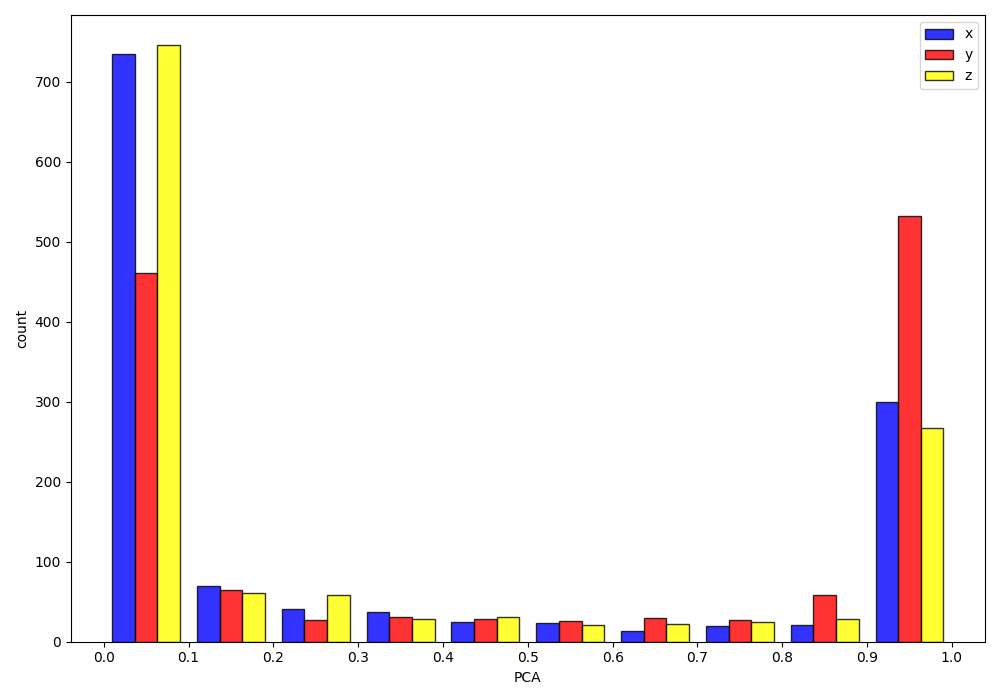
\includegraphics[width=0.5\textwidth]{picture/Initial pca}
  \caption{Value of the main eigenvector for the initial 3D mesh database}
  \label{fig:PCA-before}
  \end{center}
\end{figure}

\begin{figure}[h!]
\begin{center}
  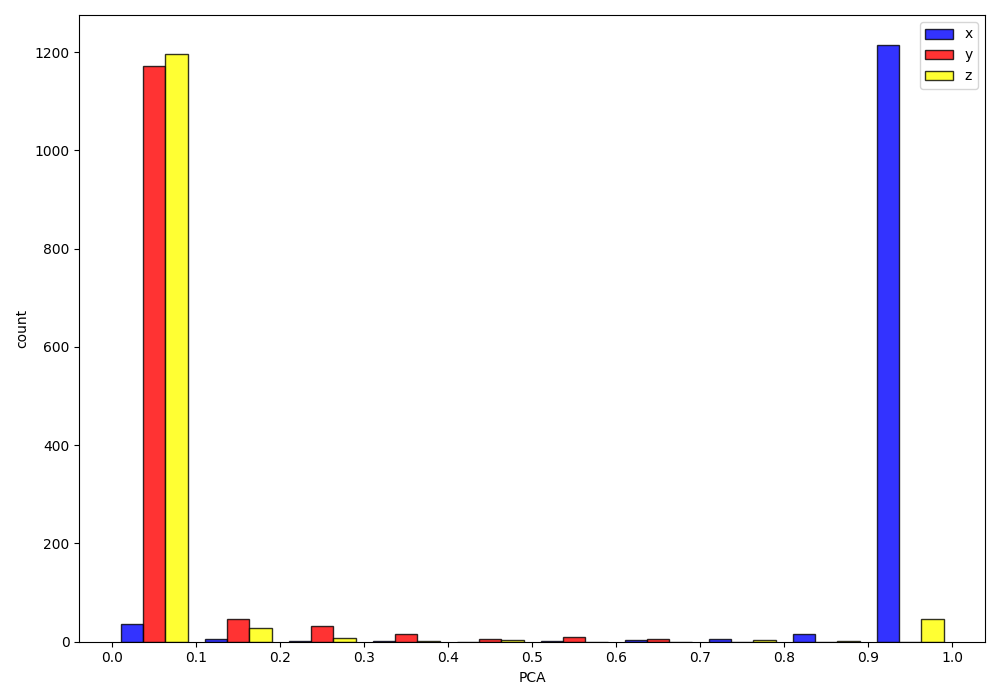
\includegraphics[width=0.5\textwidth]{picture/Normalised pca}
  \caption{Value of the main eigenvector after normalisation}
  \label{fig:PCA-after}
  \end{center}
\end{figure}
	
	We see that the axis where the vertex are the most spread is aligned with the x-axis after normalization. It means that after normalization the main eigenvector given by the PCA looks like (1,0,0) therefore the mesh is oriented as expected.
	
\subsection{Orientation}
	We now need to normalize the orientation. Determine if flipping along an axis is needed based on the moment test. We compute the second-order moment of the area with respect to a given axis, if it is negative we rotate the mesh of 180° around this axis to inverse the momentum.
	The second-order moment of the area with respect to a given axis is computed with this given formula :
	$$ f_i = \sum_{t} sign(c_{t,i})(c_{t,i})^2  $$ (with $c_{t,i}$ the i-th coordinate of center of triangle T ($i \in \{x,y,z\}$)
	

\subsection{Scaling}
	The objective here is to scale the mesh to fit in the unit cube of the 3D space. As we want all axis to be scaled with the coefficient it means that the longest side of the bounding box has to be one and the other might be lower or equal (in the case of a cube bounding box).
	We compute two points that will describe the bounding box as follows:
	$$min\_box = (\underset{v \in V}{min}(v_x),\underset{v \in V}{min}(v_y),\underset{v \in V}{min}(v_z)) $$ and $$max\_box = (\underset{v \in V}{max}(v_x), \underset{v \in V}{max}(v_y), \underset{v \in V}{max}(v_z)$$ with V the set of vertex of the mesh.
	We define the length of the bounding box as following, and for the rest of the report :
	$$ |Bounding\_box| = max(\underset{v \in V}{max\_box_i}) - \underset{v \in V}{max\_box_i}))$$ (with i the i-th coordinate of v ($i \in \{x,y,z\}$)and V the set of vertex of the mesh.)
	The definition match what we can call the longest side of the bounding box. The normalize this length to one we multiply each vertex by the inverse of the longest side of the bounding box to scale the side to one. We can observe the effect of the transformation in Figure \ref{fig:box-size-after}.

\begin{figure}[h!]
\begin{center}
  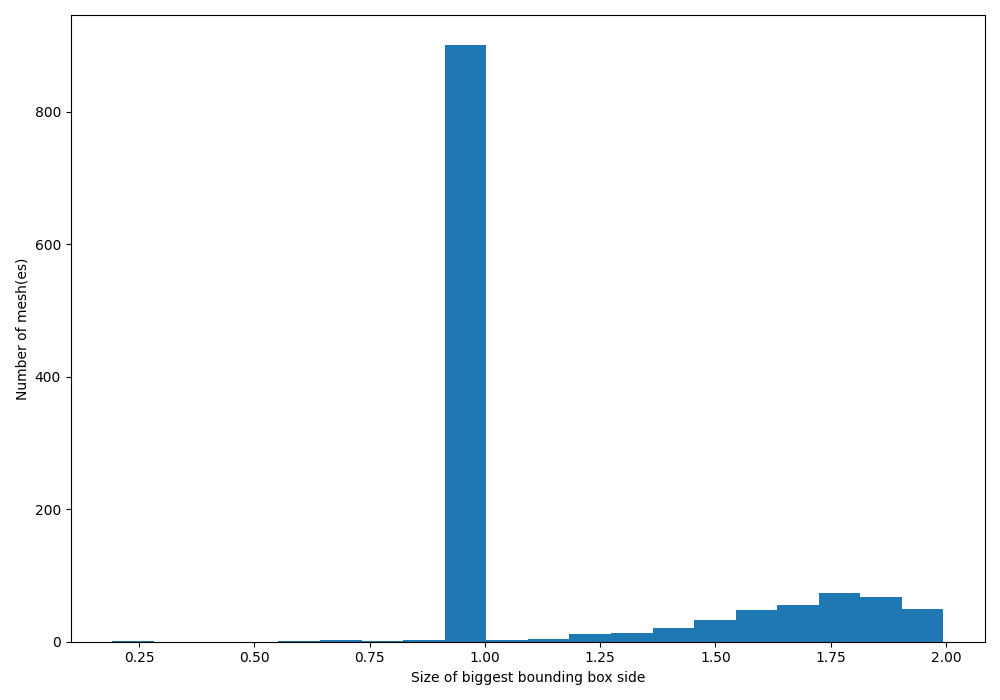
\includegraphics[width=0.5\textwidth]{picture/Initial size of biggest bounding box side}
  \caption{size of biggest bounding box side for the initial 3D mesh database}
  \label{fig:box-size-before}
  \end{center}
\end{figure}

\begin{figure}[h!]
\begin{center}
  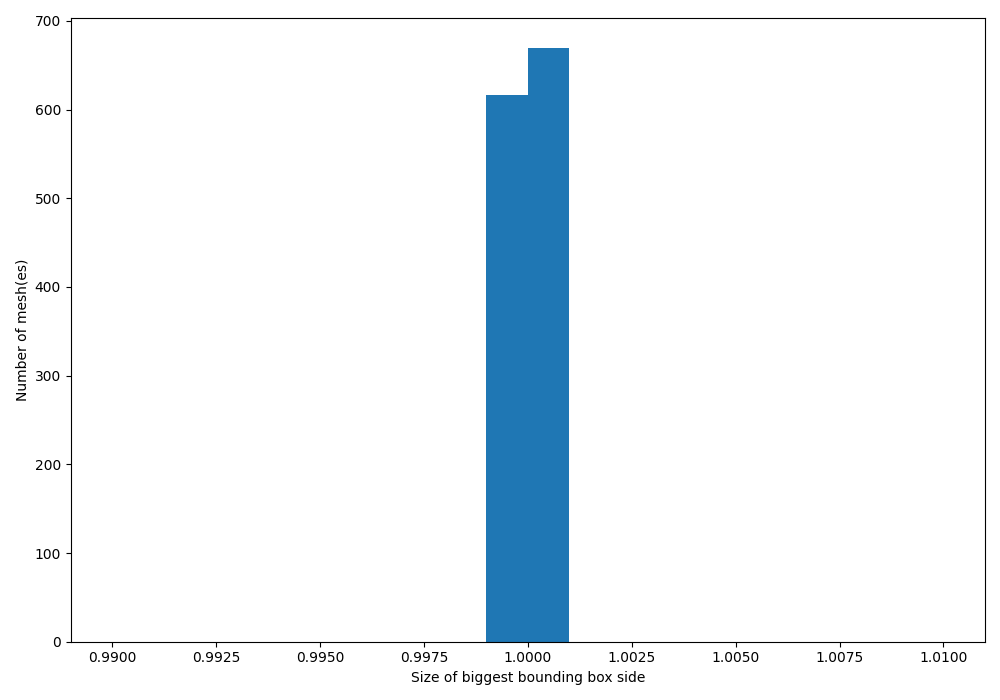
\includegraphics[width=0.5\textwidth]{picture/Normalised size of biggest bounding box side}
  \caption{Size of biggest bounding box side after normalisation}
  \label{fig:box-size-after}
  \end{center}
\end{figure}

In comparison, with the initial Database (see Figure \ref{fig:box-size-before}) we can deduce that the size of the bounding box has been normalizing around one. After an analysis, we have seen that every mesh has the size of its bounding box in $1\pm 1^{-6}$ which might be caused by the imprecision of python computing the inverse of the initial size of the bounding box.

%\section*{Acknowledgements}
%Anyone to thank/credit for helping your team along the way? This is the place to do it.
\medskip
\printbibliography
\end{document}